% !TEX root = 99_main.tex

The experiment consisting of 15 users each equipped with a fitbit over a month, produced a dataset of [INSERT NUMBER HERE] data points. Each data point is effectively a survey of the user at a particular time. The results presented in this section is intended as a demonstration of the type of analysis that can be conducted using data acquired from the cozie watch-face.


\subsection{Evaluational of User Comfort Over Day}

Figure \ref{fig:hourPlot} details a simple heat-map where the user comfort feedback is mapped to the hour of the day. Users appear to be comfortable on average [INSERT NUMEBR HERE] \% of the time, and there are no statistically significant trends during working hours (9:00 - 17:00). Variations in user comfort feedback during the day can be used to infer faulty building operation.\\

It is interesting to note that there is on average [INSERT NUMBER HERE] times more responses in the hours of 9:00, 11:00, 13:00, 15:00, and 17:00 which is when the occupant is buzzed and asked to give feedback. Nevertheless there are still significant amounts of responses made outside these times which had been done from the motivation of the participants themselves. Figure \ref{fig:responseRate} details the daily responses from the participants. Interestingly, there appears to be no trace of survey fatigue as the number of responses during the month, which includes the self-motivated responses does not decrease.

\begin{figure}
\begin{center}
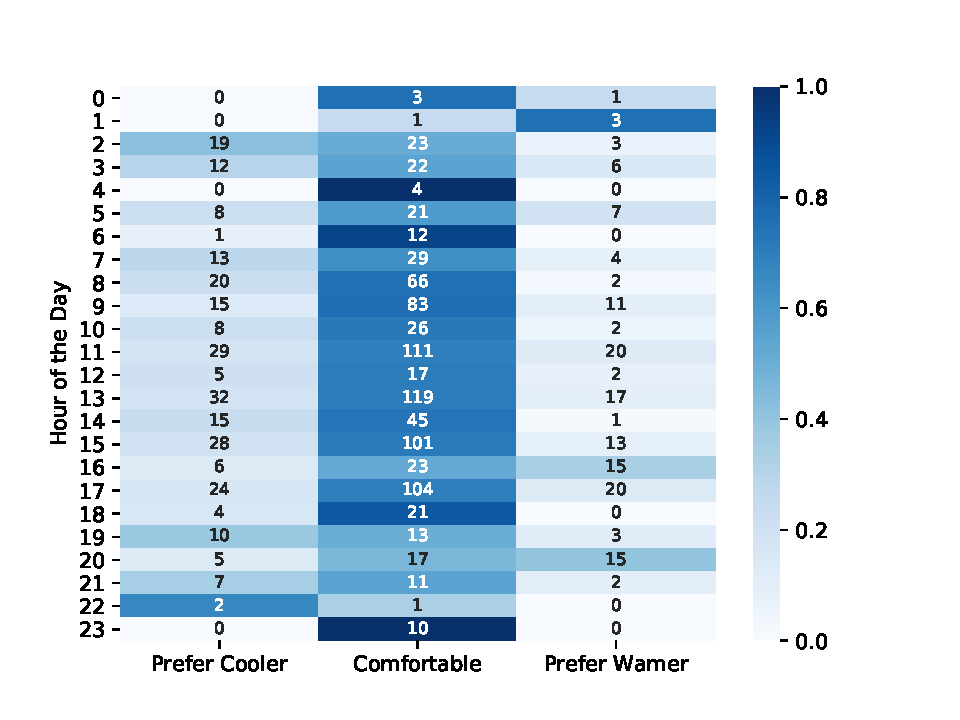
\includegraphics[width=\textwidth, trim= 0cm 0cm 0cm 0cm,clip]{hourPlot.pdf}
\caption{Aggregation of user feedback mapped to the hour of the day that feedback was given. Annotations withing the heat-map detail the absolute response value, while the colour gradient relates to the normalised values}
\label{fig:hourPlot}
\end{center}
\end{figure}

\begin{figure}
\begin{center}
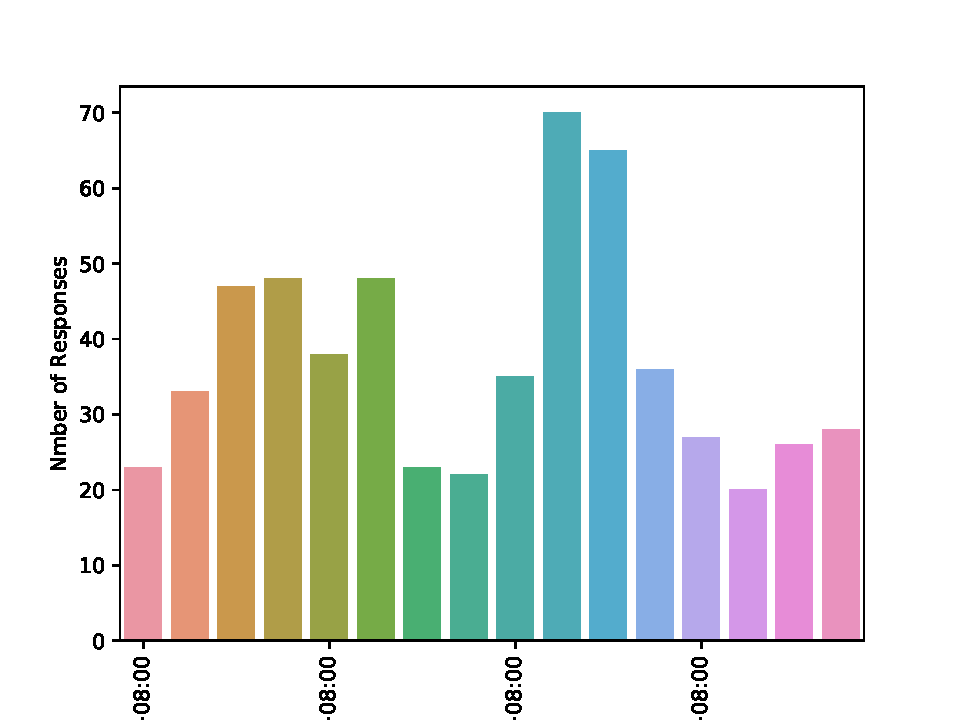
\includegraphics[width=\textwidth, trim= 0cm 0cm 0cm 0cm,clip]{response_rate.pdf}
\caption{Daily responses during the course of the evaluation period}
\label{fig:responseRate}
\end{center}
\end{figure}

\subsection{Influence of Individual Users}

Individual user feedback can be clustered using un-supervised learning techniques. In this example, we use a hierarchal k-means clustering based on euclidean distance using the Nearest-Point-Algorithm. The results, shown in Figure \ref{fig:userPlot}, show four distinct clusters of users. Users that are comfortable 100\% of the time, users that are comfortable 60-80 \% of the time, those that are comfortable 50\% of the time and generally would prefer it cooler, those that are comfortable 50\% of the time and would prefer it both warmer and cooler. Understanding and defining these differences in user preferences can be used to recommend spaces that may better suit the needs of the occupant. For example, User 5 and User 10 can be recommended working spaces that are on average cooler. User 13 on the other hand appears to have a broad comfort spectrum. 

It is important to note here that the data is not entirely representative of a single building space, as the user may have given feedback while having lunch outside. As seen in Figure \ref{fig:hourPlot}, there are even feedback results outside of working hours. Conclusions such as "Building Zone A was comfortable 80\% of the time" can therefore not be made. This will be further discussed in Section \ref{ch:discussion}.


\begin{figure}
\begin{center}
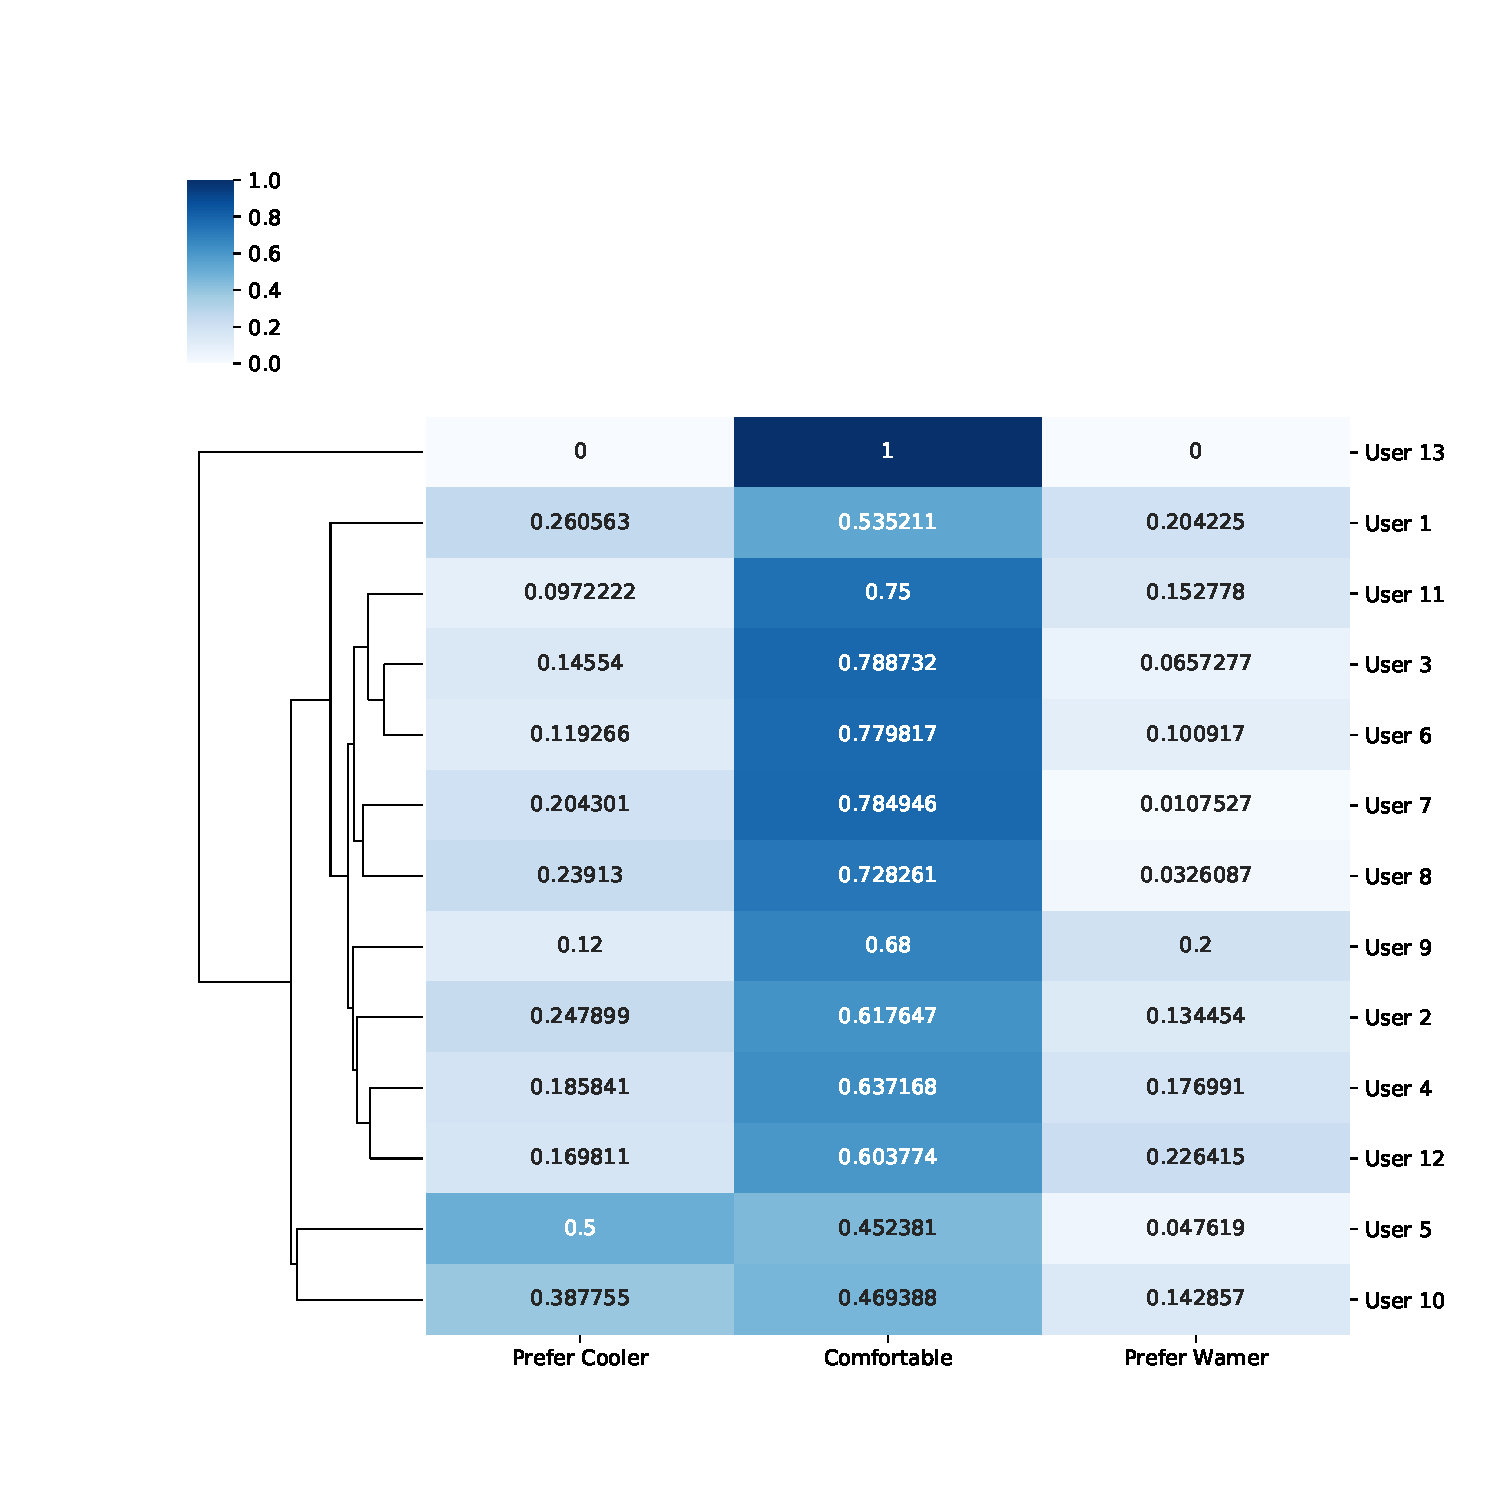
\includegraphics[width=\textwidth, trim= 0cm 0cm 0cm 0cm,clip]{cozie_users.pdf}
\caption{Clustering of user feedback using hierarchal k-means. The results show four distinct clusters.}
\label{fig:userPlot}
\end{center}
\end{figure}

\subsection{Influence of Heart-Rate}

\subsection{Combination with Sensor Data}